\documentclass[english,serif,mathserif,xcolor=pdftex,dvipsnames,table]{beamer}
% \usetheme{gc3}
\usepackage{gc3}


\title[GC3Pie]{%
  GC3Pie: \\
  orchestrating \\ large-scale execution \\ of scientific applications
}
\author[R.~Murri]{%
  \textbf{Riccardo Murri}, Sergio Maffioletti \\
  S3IT: Service and Support for Science IT, \\
  University of Zurich
}
\date{HPC-CH, June~11, 2015}

\begin{document}

% title frame
\maketitle

\begin{frame}
  \begin{center}
    \bfseries\huge
    {Let's start with an example}
  \end{center}
\end{frame}


\begin{frame}
  \begin{center}
    \textbf{Soil Mites Population Dynamics}
  \end{center}

  \begin{quote}
    Test which experimental designs give the most powerful data, by:
    \begin{itemize}
    \item simulating soil mite population dynamics and observations of
      those dynamics in different experimental designs,
    \item fitting a Bayesian statistical model to the observed data to
      estimate the rates that govern the population dynamics.
    \end{itemize}
  \end{quote}

  \begin{center}
    \+ Mollie Brooks, \url{http://www.popecol.org/}
  \end{center}
\end{frame}

\begin{frame}
  \frametitle{Scaling out from local experiment}
  \begin{itemize}
  \item Code is an R function that performs the statistical computations.
  \item Typical run on one parameter set takes between 1 and 8 hours
    on a 4-core processor.
    \pause
  \item Three sets of input parameters:
    \begin{itemize}
    \item sampling parameters (22 rows),
    \item isolation parameters (4 rows),
    \item detection parameters (11 rows).
    \end{itemize}
    \pause
  \item Need to run the same function on each combination of
    parameters\ldots
  \item \ldots and repeat 100 times for statistical significance.
  \end{itemize}

    \pause
  \begin{center}
    {\bf So it's 96800 runs, \\ totalling circa 1'600'000 core hours.}
  \end{center}
\end{frame}

\begin{frame}[fragile]
  \frametitle{How does GC3Pie help? \em (1)}

  \begin{center}
    Write a Python script to drive execution!
  \end{center}

  \begin{lstlisting}[showstringspaces=false,basicstyle=\tiny\ttfamily]
class GmbsimScript(SessionBasedScript):
  """
  Read the specified INPUT ``.csv`` files and submit jobs according
  to the content of those files.
  """
  # \ldots setup command-line options etc \ldots
  def new_tasks(self, extra):
    # read list of parameter sets from input files
    dates_and_sampling_exps = read_param_file(self.params.sampling)
    isolation_exps = read_param_file(self.params.isolation)
    detection_exps = read_param_file(self.params.detection)
    # loop over data to create jobs
    for date_and_sampling, isolation, detection in \
            product(dates_and_sampling_exps, isolation_exps, detection_exps):
      # \ldots prepare data and job description \ldots
      for n in range(1, self.params.replicates):
        yield GmbsimApplication(
          scriptfile=self.params.scriptfile,
          datafiles=self.params.datafiles,
          days_of_the_week=dates,
          sampling_exp=sampling,
          isolation_exp=isolation,
          detection_exp=detection,
          @\ldots@)
  \end{lstlisting}
\end{frame}


\begin{frame}[fragile]
  \frametitle{How does GC3Pie help? \em (2)}

  \begin{lstlisting}[language=sh,basicstyle=\scriptsize\ttfamily]
@\bfseries ./gmbsim.py 100 sampling.csv isolation2.csv detection.csv@ \
  @\bfseries sim\_run\_dclone\_design\_test3.R weird\_dates\_sdur.R@ \
  @\bfseries -s take4 -C 600 -J 500 -w '72 hours' -c 4@
# ...
Status of jobs in the 'take4' session: (at 01:25:10, 05/12/15)
         NEW  4764/9600   (49.62%)
     RUNNING   216/9600   (2.25%)
     STOPPED     0/9600   (0.00%)
   SUBMITTED   284/9600   (2.96%)
  TERMINATED  4336/9600   (45.17%)
 TERMINATING     0/9600   (0.00%)
     UNKNOWN     0/9600   (0.00%)
       total  9600/9600  (100.00%)
     \end{lstlisting}
\end{frame}


\begin{frame}
  \begin{center}
    \bfseries\huge
    {What is {\em GC3Pie} and \\ why do we need something like that ?}
  \end{center}
\end{frame}


% \begin{frame}
%   \frametitle{Workflow management}

%   \begin{center}
%     \emph{Automate} execution \\ of a large number of \emph{different
%       applications} \\ on a \emph{variety of computational resources.}
%   \end{center}
% \end{frame}

% \begin{frame}
%   \frametitle{Workflow management, \em (2)}

%   \begin{enumerate}
%   \item{\textbf{Access}} to computational resources
%   \item{\textbf{Supervise}} execution of collection of jobs
%   \item{\textbf{Handling}} of error conditions individually
%   \item{\textbf{Post-process}} and store results
%   \end{enumerate}
% \end{frame}


\begin{frame}
  \frametitle{What is GC3Pie then?}
  GC3Pie is \ldots
  \begin{enumerate}
  \item<1-> \alert<1>{An \emph{opinionated} Python framework for defining and running computational workflows;}
  \item<2-> \alert<2>{A \emph{rapid development toolkit} for enabling user applications run unmodified on clusters and IaaS cloud resources;}
  \item<3-> \alert<3>{The worst name ever given to a middleware piece\ldots}
  \end{enumerate}
\end{frame}


\begin{frame}
  \frametitle{The issues GC3Pie wants to solve}
  \begin{enumerate}
  \item \textbf{Portability:} Run on a different computing
    infrastructure without rewriting all the scripts.
  \item \textbf{Code reuse:} Scripts are often very tied to a certain
    purpose, so they are difficult to reuse.
  \item \textbf{Heavy maintenance:} the more a script does its job
    well, the more you'll find yourself adding \emph{generic} features
    and maintaining requests from other users.
  \end{enumerate}
\end{frame}


\begin{frame}
  \begin{center}
    {\bfseries\huge
      {High-level architecture overview}}
    \\ \+
    Again, let's do this through an example.
  \end{center}
\end{frame}


\begin{frame}
  \frametitle{High-level architecture}
  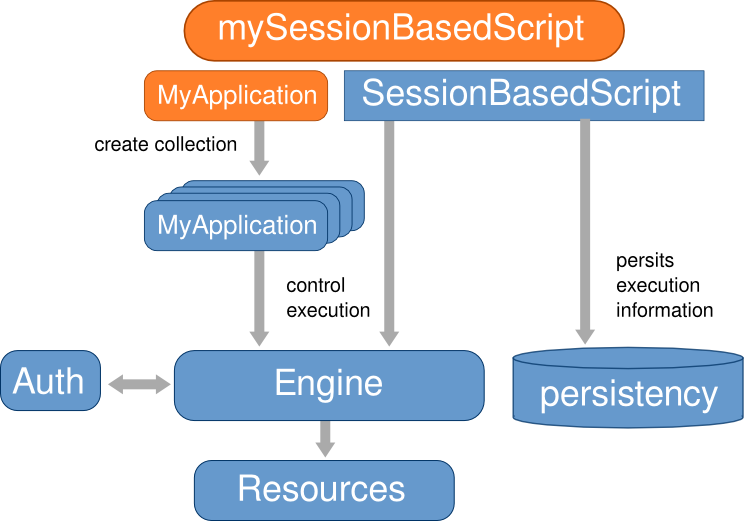
\includegraphics[width=0.8\textwidth]{fig/GC3Pie_execution_model}
\end{frame}

\begin{frame}[fragile]
  \begin{center}
    An application is a subclass of the \texttt{gc3libs.Application}
    class.
  \end{center}
  \begin{lstlisting}[showstringspaces=false,basicstyle=\tiny\ttfamily]
class GmbsimScript(SessionBasedScript):
  # \ldots
  def new_tasks(self, extra):
    @\ldots@
    # loop over data to create jobs
    for date_and_sampling, isolation, detection in \
            product(dates_and_sampling_exps, isolation_exps, detection_exps):
      # \ldots prepare data and job description \ldots
      for n in range(1, self.params.replicates):
        yield @\HL{GmbsimApplication}@(
          scriptfile=self.params.scriptfile,
          datafiles=self.params.datafiles,
          days_of_the_week=dates,
          sampling_exp=sampling,
          isolation_exp=isolation,
          detection_exp=detection,
          @\ldots@)
\end{lstlisting}
\end{frame}

\begin{frame}[fragile]
  \begin{center}
    Applications can be grouped into \emph{collections}.
  \end{center}
  \begin{lstlisting}[showstringspaces=false,basicstyle=\tiny\ttfamily]
class GmbsimScript(SessionBasedScript):
  # \ldots
  def new_tasks(self, extra):
    @\ldots@
    # loop over data to create jobs
    @\HL{for date\_and\_sampling, isolation, detection in}@ \
        product(dates\_and\_sampling\_exps, isolation\_exps, detection\_exps):
      # \ldots prepare data and job description \ldots
      @\HL{for n in range(1, self.params.replicates):}@
        yield GmbsimApplication(
          scriptfile=self.params.scriptfile,
          datafiles=self.params.datafiles,
          days_of_the_week=dates,
          sampling_exp=sampling,
          isolation_exp=isolation,
          detection_exp=detection,
          @\ldots@)
  \end{lstlisting}
\end{frame}

\begin{frame}
  \frametitle{High-level architecture: \texttt{Engine}}
  \begin{columns}
    \begin{column}{0.5\textwidth}
      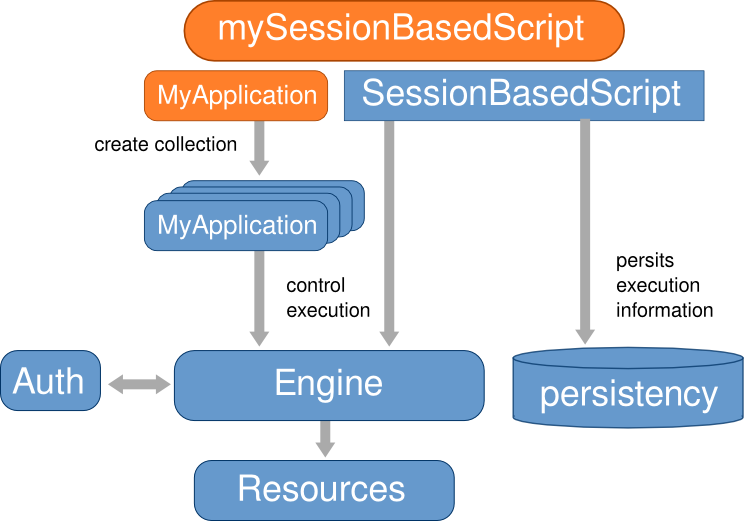
\includegraphics[width=1\textwidth]{fig/GC3Pie_execution_model}
    \end{column}
    \begin{column}{0.6\textwidth}
      \begin{flushright}
        Execution of applications and collections is delegated to an
        \texttt{Engine}.
      \end{flushright}
    \end{column}
  \end{columns}
\end{frame}

\begin{frame}
  \frametitle{High-level architecture: resources}
  \begin{columns}
    \begin{column}{0.5\textwidth}
      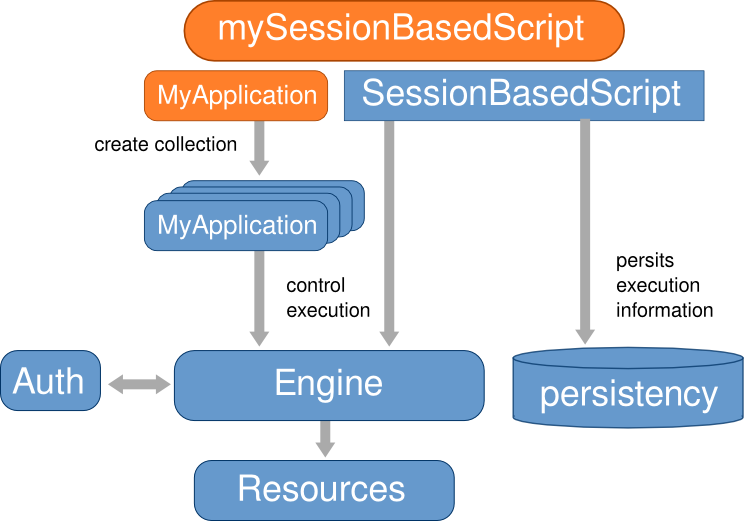
\includegraphics[width=1\textwidth]{fig/GC3Pie_execution_model}
    \end{column}
    \begin{column}{0.6\textwidth}
      \begin{flushright}
    %   A \emph{Resource} is a computational endpoint where the
    %   execution of the {\it Application} takes place.

        GC3Pie can execute applications on a variety of resources:
        \alert<2>{\em cloud-based VMs,} \\
        \alert<3>{\em batch-queueing clusters}, and \\
        \alert<4>{any~host~which~you~can~\texttt{ssh}~to.}

        \+ The \texttt{Engine} handles the access to computational {\em
          resources} transparently.
      \end{flushright}
    \end{column}
  \end{columns}
\end{frame}


\begin{frame}
  \frametitle{High-level architecture: \texttt{SessionBasedScript}}
  \begin{columns}
    \begin{column}{0.5\textwidth}
      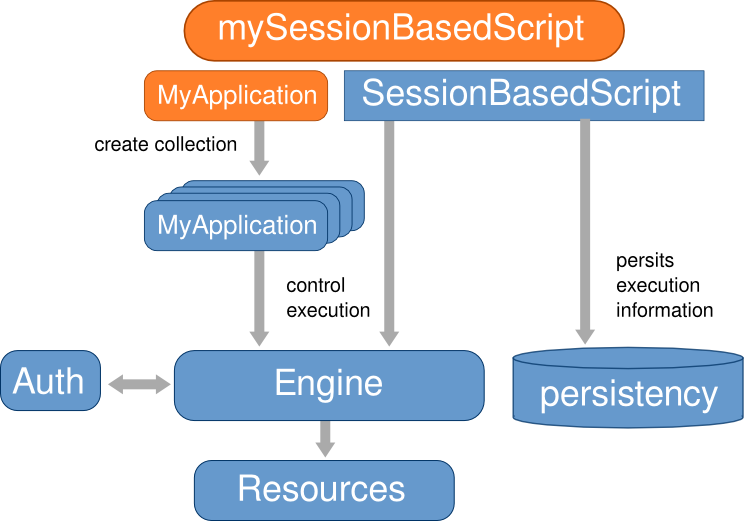
\includegraphics[width=1\textwidth]{fig/GC3Pie_execution_model}
    \end{column}
    \begin{column}{0.6\textwidth}
      \begin{flushright}
        A convenient {\em SessionBasedScript} class contains already
        most of the control logic for instructing the execution
        engine.

        \+ The \texttt{SessionBasedScript} takes also care of {\em
          persisting} execution information.
      \end{flushright}
    \end{column}
  \end{columns}
\end{frame}


\begin{frame}[fragile]
  \begin{center}
    To create a script just subclass \texttt{SessionBasedScript}.
  \end{center}
  \begin{lstlisting}[showstringspaces=false,basicstyle=\tiny\ttfamily]
@\HL{class GmbsimScript(SessionBasedScript):}@
  # \ldots
  def new_tasks(self, extra):
    @\ldots@
    # loop over data to create jobs
    for date\_and\_sampling, isolation, detection in \
        product(dates\_and\_sampling\_exps, isolation\_exps, detection\_exps):
      # \ldots prepare data and job description \ldots
      for n in range(1, self.params.replicates):
        yield GmbsimApplication(
          scriptfile=self.params.scriptfile,
          datafiles=self.params.datafiles,
          days_of_the_week=dates,
          sampling_exp=sampling,
          isolation_exp=isolation,
          detection_exp=detection,
          @\ldots@)
  \end{lstlisting}
\end{frame}


\begin{frame}[fragile]
  \begin{center}
    Customization is done by overriding specific methods.
  \end{center}
  \begin{lstlisting}[showstringspaces=false,basicstyle=\tiny\ttfamily]
class GmbsimScript(SessionBasedScript):
  # \ldots
  @\HL{def setup\_options(self):}@
    self.add_param("-b", "-nb", "--burn-in", metavar="NUM",
             dest="nb", default=1,
             help="Execute NUM iterations for JAGS burn-in.")
    self.add_param("-i", "-ni", "--iter", metavar="NUM",
             dest="ni", default=3,
             help="Execute NUM JAGS main iterations.")
    @\ldots@
    # change default for the core/memory/walltime options
    self.actions['memory_per_core'].default = 1*Memory.GB
    self.actions['wctime'].default = '2 hours'
    self.actions['ncores'].default = 4
  \end{lstlisting}
\end{frame}


\begin{frame}[fragile]
  \frametitle{\texttt{SessionBasedScript} example}
\begin{lstlisting}[language=sh,basicstyle=\tiny\ttfamily]
$ @\bfseries ./gmbsim.py --help@
usage: gmbsim [-h] [-V] [-v] [--config-files CONFIG_FILES] [-c NUM]
              [-m GIGABYTES] [-r NAME] [-w DURATION] [-s PATH] [-u URL] [-N]
              [-C NUM] [-J NUM] [-o DIRECTORY] [-l [STATES]] [-b NUM] [-i NUM]
              [-t NUM]
              replicates sampling isolation detection scriptfile
              [datafiles [datafiles ...]]
\end{lstlisting}% $
\end{frame}


\begin{frame}
  \begin{center}
    \bfseries\huge
    {From single tasks \\ to workflows}
  \end{center}
\end{frame}


\begin{frame}
\frametitle{Task dependency management}
\begin{center}
    An \texttt{Engine} manages all jobs concurrently. \\
    What if there are inter-application dependencies?
    \\ \+
    GC3Pie provides {\em Task composition} support (workflow), created
    programmatically from Python code.
    \\ \+
    Which means, no graphical editor.  But also means you can create
    workflows {\em on-the-fly} as your computation proceeds.
\end{center}
\end{frame}


\begin{frame}
\frametitle{Example: EasyBuild}
\begin{columns}
  \begin{column}{0.4\linewidth}
    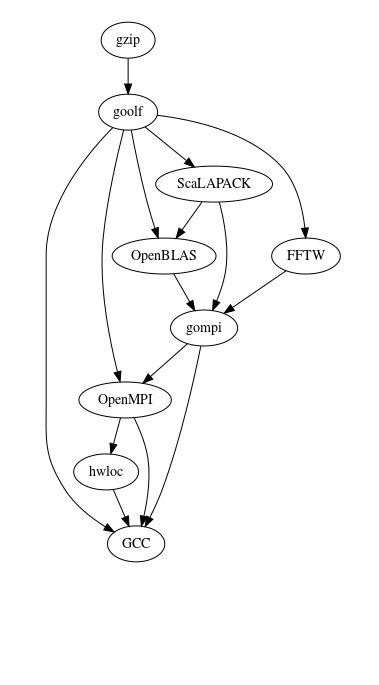
\includegraphics[height=1.00\textheight]{fig/gzip1.png}
  \end{column}
  \begin{column}{0.6\linewidth}
    \begin{flushright}
      EasyBuild has built-in dependency resolution.  To compile
      \texttt{gzip} you first have to build another 8 software
      packages.

      \+
      Starting with version 2.2, EasyBuild can launch all these
      compilation jobs through GC3Pie.
    \end{flushright}
  \end{column}
\end{columns}
\end{frame}


\begin{frame}[fragile]
  \frametitle{Dependency-based task management}
  \begin{columns}
    \begin{column}{0.4\linewidth}
      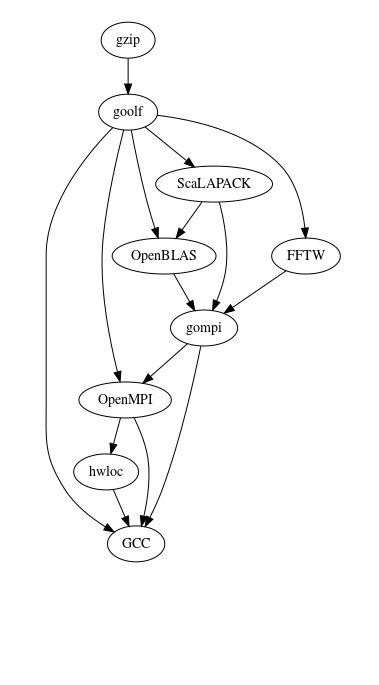
\includegraphics[height=1.00\textheight]{fig/gzip1.png}
    \end{column}
    \begin{column}{0.6\linewidth}
      \begin{flushleft}
        Code-wise this is easy.  Create a
        \texttt{DependentTaskCollection} and tell it what tasks it has
        to run and the dependencies of each.
        \\ \+
\begin{semiverbatim}\small
coll = DependentTaskCollection()
coll.add(gzip_task, [goolf_task])
coll.add(goolf_task, [
  gcc_task,
  fftw_task,
  scalapack_task
])
\ldots
\end{semiverbatim}
      \end{flushleft}
    \end{column}
  \end{columns}
\end{frame}


\begin{frame}[fragile]
  \frametitle{Parallel task management}
  \begin{columns}
    \begin{column}{0.4\linewidth}
      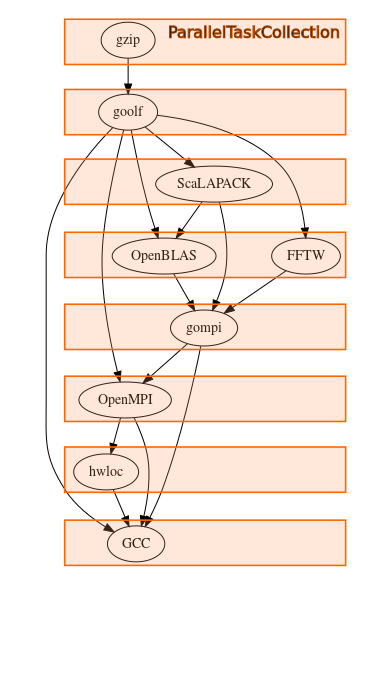
\includegraphics[height=1.00\textheight]{fig/gzip2.png}
    \end{column}
    \begin{column}{0.6\linewidth}
      \begin{flushright}
        Under the hood, GC3Pie groups independent tasks into a
        \texttt{ParallelTaskCollection}.
        \\ \+
        This means they can run independently.
      \end{flushright}
    \end{column}
  \end{columns}
\end{frame}


\begin{frame}[fragile]
  \frametitle{Sequencing tasks}
  \begin{columns}
    \begin{column}{0.4\linewidth}
      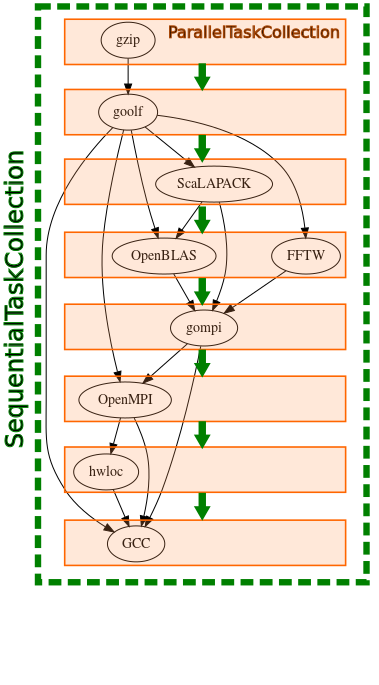
\includegraphics[height=1.00\textheight]{fig/gzip3.png}
    \end{column}
    \begin{column}{0.6\linewidth}
      \begin{flushright}
        Several tasks and task collections can be forced to run in a
        sequence using a \texttt{SequentialTaskCollection}.
      \end{flushright}
    \end{column}
  \end{columns}
\end{frame}


\begin{frame}[fragile]
  \frametitle{Sequencing tasks, II}
  \begin{center}
    The interesting thing about \texttt{SequentialTaskCollection} \\
    is that it can be built ``lazily'' while it runs.
    \\ \+
    In other words, not all tasks need to be known \\ when the workflow
    starts running.
    \\ \+
    For example, GC3Pie sports a \emph{differential evolution}
    numerical optimizer built using this mechanism.
  \end{center}
\end{frame}


\begin{frame}
  \frametitle{References}
  \begin{center}
    Read more: \url{http://gc3pie.readthedocs.org/}

    \+\+\+ {\Large Thank you for your attention!}
  \end{center}
\end{frame}

\begin{frame}
  \frametitle{We're renaming!}

  \Large\centering
  Help choose a better name for GC3Pie!
  \\ \+
  Send suggestions and cast your vote at:
  \url{http://tinyurl.com/gc3pie-rename}
\end{frame}


\part{Additional material}

\begin{frame}
  \frametitle{GC3Pie (SW) users}
  \begin{center}
    \href{http://github.com/pelkmanslab/iBRAIN_UZH}{iBRAIN} -- High-throughput screening framework, Pelkmans Lab UZH.
    \\ \+
    \href{http://huygens-remote-manager.readthedocs.org/en/latest/}{Huygens Remote Manager} -- Web-based interface \\ to Huygens Core for multi-user \\ batch-scheduled deconvolution.
    \\ \+
    \href{http://www.ncbi.nlm.nih.gov/pubmed/25987568}{TRAL} -- the \emph{Tandem Repeat Annotation Library}, \\ Elke Schaper (ISB-SIB) et al.
  \end{center}
\end{frame}


\end{document}

%%% Local Variables:
%%% mode: latex
%%% TeX-master: t
%%% End:
